\newcommand{\wormTagResultsAucTable}{
    \begin{table}[H]
        \centering
        \begin{tabular}{|p{2,8cm}||P{2,2cm} P{2,2cm} P{2,2cm} P{2,2cm}|}
            \hline
            Worm Tag & ALOHA\newline (M/B only) & ALOHA & Joint\newline Embedding & Proposed\newline Model \\
            \hline
            AUC-ROC & - & \textBF{0.966$\pm$0.010} & 0.928$\pm$0.014 & 0.940$\pm$0.014 \\
            \hline
        \end{tabular}
        \caption[Worm Tag prediction task AUC-ROC results]{AUC-ROC (Area Under Curve) of the different models for the \textbf{Worm Tag} prediction task. Results were aggregated over \textBF{3} training runs with different weight initializations and minibatch orderings. Best results are shown in \textbf{bold}.} \label{tab:wormTag_auc}
    \end{table}
}

\newcommand{\wormTagResultsAtFprTable}{
    \begin{center}
        \begin{longtable}[c]{|P{3,2cm}||P{1,8cm} P{1,8cm} P{1,8cm} P{1,8cm} P{1,8cm}|}
            \hline
            Worm Tag & \multicolumn{5}{c|}{{FPR}} \\
            & $10^{-5}$ & $10^{-4}$ & $10^{-3}$ & $10^{-2}$ & $10^{-1}$ \\
            \hline
            \endfirsthead

            \caption*{\raggedright ...continued from previous page} \\
            \hline
            Worm Tag & \multicolumn{5}{c|}{\textbf{FPR}} \\
            & $10^{-5}$ & $10^{-4}$ & $10^{-3}$ & $10^{-2}$ & $10^{-1}$ \\
            \hline
            \endhead

            \caption*{\raggedleft ...continued on next page} \\
            \endfoot

            \caption[Worm Tag prediction task results]{Mean and standard deviation results (TPR, Accuracy, Recall, Precision and F1-Score) of the different models for the \textbf{Worm Tag} prediction task at different \textbf{FPR}s (\textit{False Positive Rates}). Results were aggregated over \textBF{3} training runs with different weight initializations and minibatch orderings. Best results are shown in \textbf{bold}. Under \textbf{TPR} results are also presented the percentage reduction in mean detection error and in ROC curve standard deviation introduced by the \textit{Proposed Model} with respect to both \textit{ALOHA} model and \textit{Joint Embedding}.} \label{tab:wormTag_results_at_fpr} \\
            \endlastfoot

            \multicolumn{6}{|c|}{\textbf{TPR}} \\
            \hline
            ALOHA (M/B only) & - & - & - & - & - \\
            ALOHA & 0.004$\pm$0.003 & 0.062$\pm$0.020 & 0.289$\pm$0.108 & 0.605$\pm$0.012 & \textBF{0.877$\pm$0.061} \\
            Joint Embedding & \textBF{0.117$\pm$0.035} & 0.191$\pm$0.098 & \textBF{0.581$\pm$0.012} & 0.656$\pm$0.004 & 0.770$\pm$0.015 \\
            Proposed Model & 0.104$\pm$0.054 & \textBF{0.204$\pm$0.119} & 0.508$\pm$0.094 & \textBF{0.657$\pm$0.007} & 0.785$\pm$0.011 \\
            \hline
            Error Reduction wrt\newline ALOHA (M/B only) & - & - & - & - & - \\
            Error Reduction wrt\newline ALOHA & 10.0\% & 15.1\% & 30.8\% & 13.2\% & -74.8\% \\
            Error Reduction wrt\newline Joint Embedding & -1.5\% & 1.6\% & -17.4\% & 0.3\% & 6.5\% \\
            \hline
            Std Reduction wrt\newline ALOHA (M/B only) & - & - & - & - & - \\
            Std Reduction wrt\newline ALOHA & -1700.0\% & -495.0\% & 13.0\% & 41.7\% & 82.0\% \\
            Std Reduction wrt\newline Joint Embedding & -54.3\% & -21.4\% & -683.3\% & -75.0\% & 26.7\% \\
            \hline
            \multicolumn{6}{|c|}{\textbf{Accuracy}} \\
            \hline
            ALOHA (M/B only) & - & - & - & - & - \\
            ALOHA & 0.842$\pm$0.000 & 0.851$\pm$0.003 & 0.887$\pm$0.017 & 0.929$\pm$0.002 & \textBF{0.896$\pm$0.010} \\
            Joint Embedding & \textBF{0.860$\pm$0.005} & 0.872$\pm$0.015 & \textBF{0.933$\pm$0.002} & \textBF{0.937$\pm$0.001} & 0.879$\pm$0.002 \\
            Proposed Model & 0.858$\pm$0.009 & \textBF{0.874$\pm$0.019} & 0.921$\pm$0.015 & \textBF{0.937$\pm$0.001} & 0.882$\pm$0.002 \\
            \hline
            \multicolumn{6}{|c|}{\textbf{Recall}} \\
            \hline
            ALOHA (M/B only) & - & - & - & - & - \\
            ALOHA & 0.004$\pm$0.003 & 0.062$\pm$0.020 & 0.289$\pm$0.108 & 0.605$\pm$0.012 & \textBF{0.877$\pm$0.061} \\
            Joint Embedding & \textBF{0.117$\pm$0.035} & 0.191$\pm$0.098 & \textBF{0.581$\pm$0.012} & 0.656$\pm$0.004 & 0.770$\pm$0.015 \\
            Proposed Model & 0.104$\pm$0.054 & \textBF{0.204$\pm$0.119} & 0.508$\pm$0.094 & \textBF{0.657$\pm$0.007} & 0.785$\pm$0.011 \\
            \hline
            \multicolumn{6}{|c|}{\textbf{Precision}} \\
            \hline
            ALOHA (M/B only) & - & - & - & - & - \\
            ALOHA & 0.980$\pm$0.016 & 0.990$\pm$0.004 & 0.980$\pm$0.006 & 0.919$\pm$0.002 & \textBF{0.622$\pm$0.017} \\
            Joint Embedding & \textBF{1.000$\pm$0.000} & \textBF{0.998$\pm$0.001} & \textBF{0.991$\pm$0.000} & \textBF{0.925$\pm$0.000} & 0.592$\pm$0.005 \\
            Proposed Model & 0.999$\pm$0.000 & 0.997$\pm$0.002 & 0.989$\pm$0.002 & 0.925$\pm$0.001 & 0.596$\pm$0.004 \\
            \hline
            \multicolumn{6}{|c|}{\textbf{F1 Score}} \\
            \hline
            ALOHA (M/B only) & - & - & - & - & - \\
            ALOHA & 0.009$\pm$0.005 & 0.116$\pm$0.036 & 0.436$\pm$0.124 & 0.730$\pm$0.009 & \textBF{0.727$\pm$0.033} \\
            Joint Embedding & \textBF{0.209$\pm$0.054} & 0.310$\pm$0.133 & \textBF{0.732$\pm$0.010} & 0.767$\pm$0.003 & 0.669$\pm$0.009 \\
            Proposed Model & 0.185$\pm$0.086 & \textBF{0.324$\pm$0.155} & 0.666$\pm$0.083 & \textBF{0.768$\pm$0.005} & 0.678$\pm$0.007 \\
            \hline
        \end{longtable}
    \end{center}
}

\newcommand{\wormTagResultsSummaryTable}{
    \begin{table}[H]
        \centering
        \begin{tabular}{|P{3,2cm}||P{1,8cm} P{1,8cm} P{1,8cm} P{1,8cm} P{1,8cm}|}
            \hline
            \multicolumn{6}{|c|}{Worm Tag (at FPR $=1\%$)} \\
            \hline
            Model & TPR & Accuracy & Precision & Recall & F1 score \\
            \hline
            ALOHA (M/B only) & - & - & - & - & - \\
            ALOHA & 0.605$\pm$0.012 & 0.929$\pm$0.002 & 0.919$\pm$0.002 & 0.605$\pm$0.012 & 0.730$\pm$0.009 \\
            Joint Embedding & 0.656$\pm$0.004 & \textBF{0.937$\pm$0.001} & \textBF{0.925$\pm$0.000} & 0.656$\pm$0.004 & 0.767$\pm$0.003 \\
            Proposed Model & \textBF{0.657$\pm$0.007} & \textBF{0.937$\pm$0.001} & 0.925$\pm$0.001 & \textBF{0.657$\pm$0.007} & \textBF{0.768$\pm$0.005} \\
            \hline
        \end{tabular}
        \caption[Summary of Worm Tag prediction task results]{Summary of the mean and standard deviation results of the different models for the \textbf{Worm Tag} prediction task at \textbf{FPR} $=1\%$. Results were aggregated over \textBF{3} training runs with different weight initializations and minibatch orderings. Best results are shown in \textbf{bold}.} \label{tab:wormTag_result_summary}
    \end{table}
}

\newcommand{\wormTagRocAlohaMB}{
    \begin{figure}[H]
        \vspace*{-0.5cm}
        \centering
        \includegraphics[width=0.6\textwidth]{./results/worm_tag_roc_alohaMB.png}
        \vspace*{-0.2cm}
        \caption[Worm Tag prediction task ALOHA (M/B only) ROC curve]{ROC curve and AUC statistics of \textBF{ALOHA (M/B only)} model for the \textbf{Worm Tag}. The line represents the \textit{mean} TPR at a given FPR, while the shaded region represents the \textit{standard deviation}. Statistics were computed over \textBF{3} training runs, each with random parameter initialization.}
        \label{fig:wormTagRocAlohaMB}
    \end{figure}
}

\newcommand{\wormTagRocAloha}{
    \begin{figure}[H]
        \vspace*{-0.5cm}
        \centering
        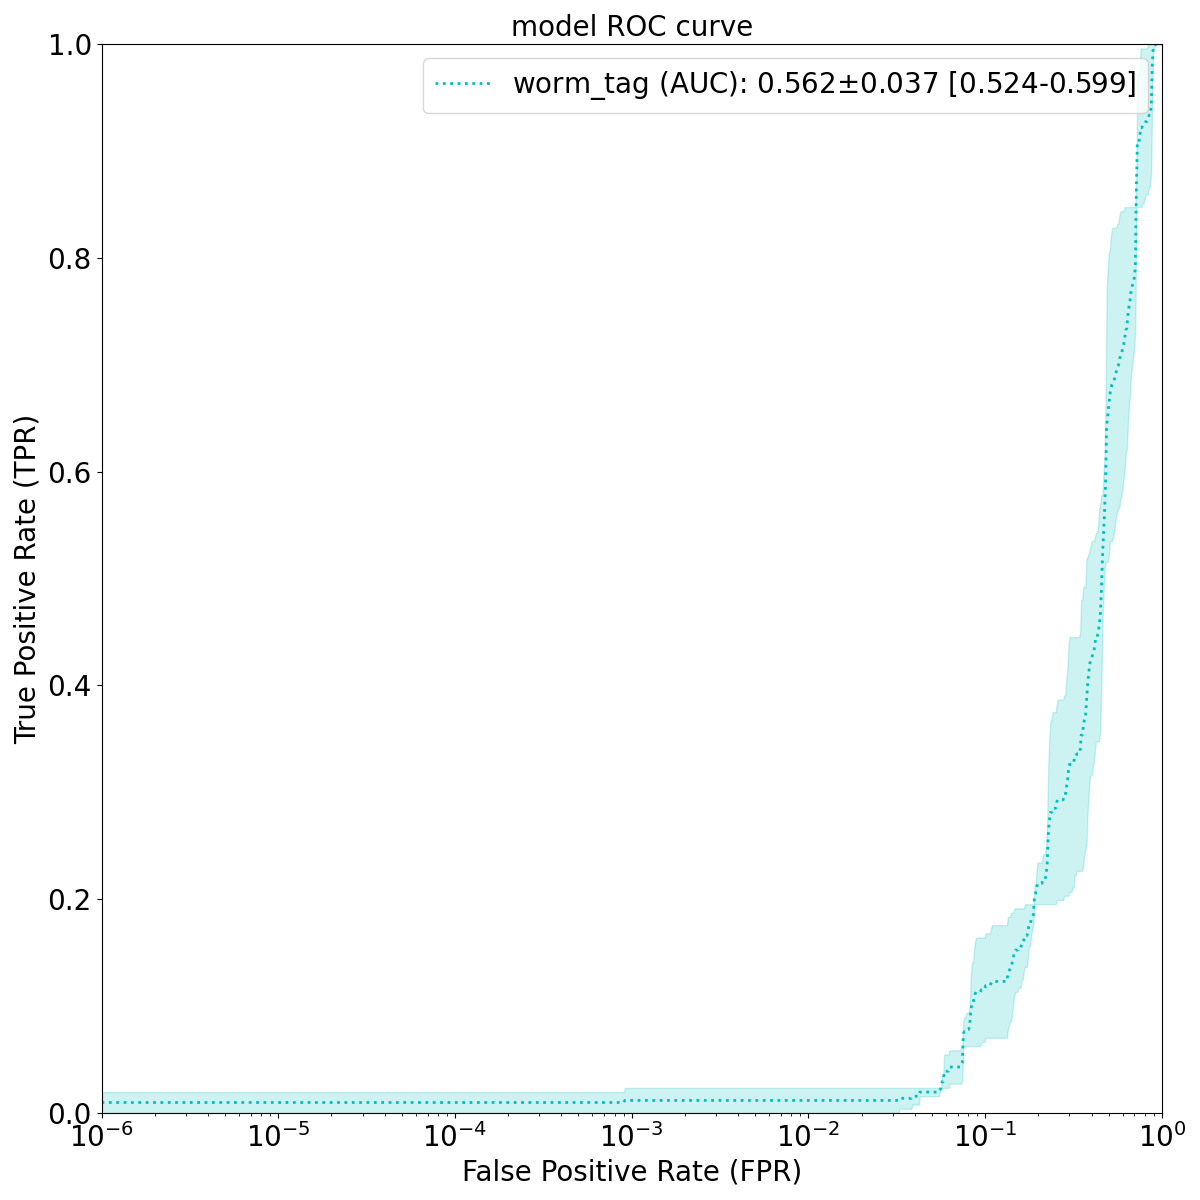
\includegraphics[width=0.6\textwidth]{./results/worm_tag_roc_aloha.png}
        \vspace*{-0.2cm}
        \caption[Worm Tag prediction task ALOHA ROC curve]{ROC curve and AUC statistics of \textBF{ALOHA} model for the \textbf{Worm Tag}. The line represents the \textit{mean} TPR at a given FPR, while the shaded region represents the \textit{standard deviation}. Statistics were computed over \textBF{3} training runs, each with random parameter initialization.}
        \label{fig:wormTagRocAloha}
    \end{figure}
}

\newcommand{\wormTagRocJointEmbedding}{
    \begin{figure}[H]
        \vspace*{-0.5cm}
        \centering
        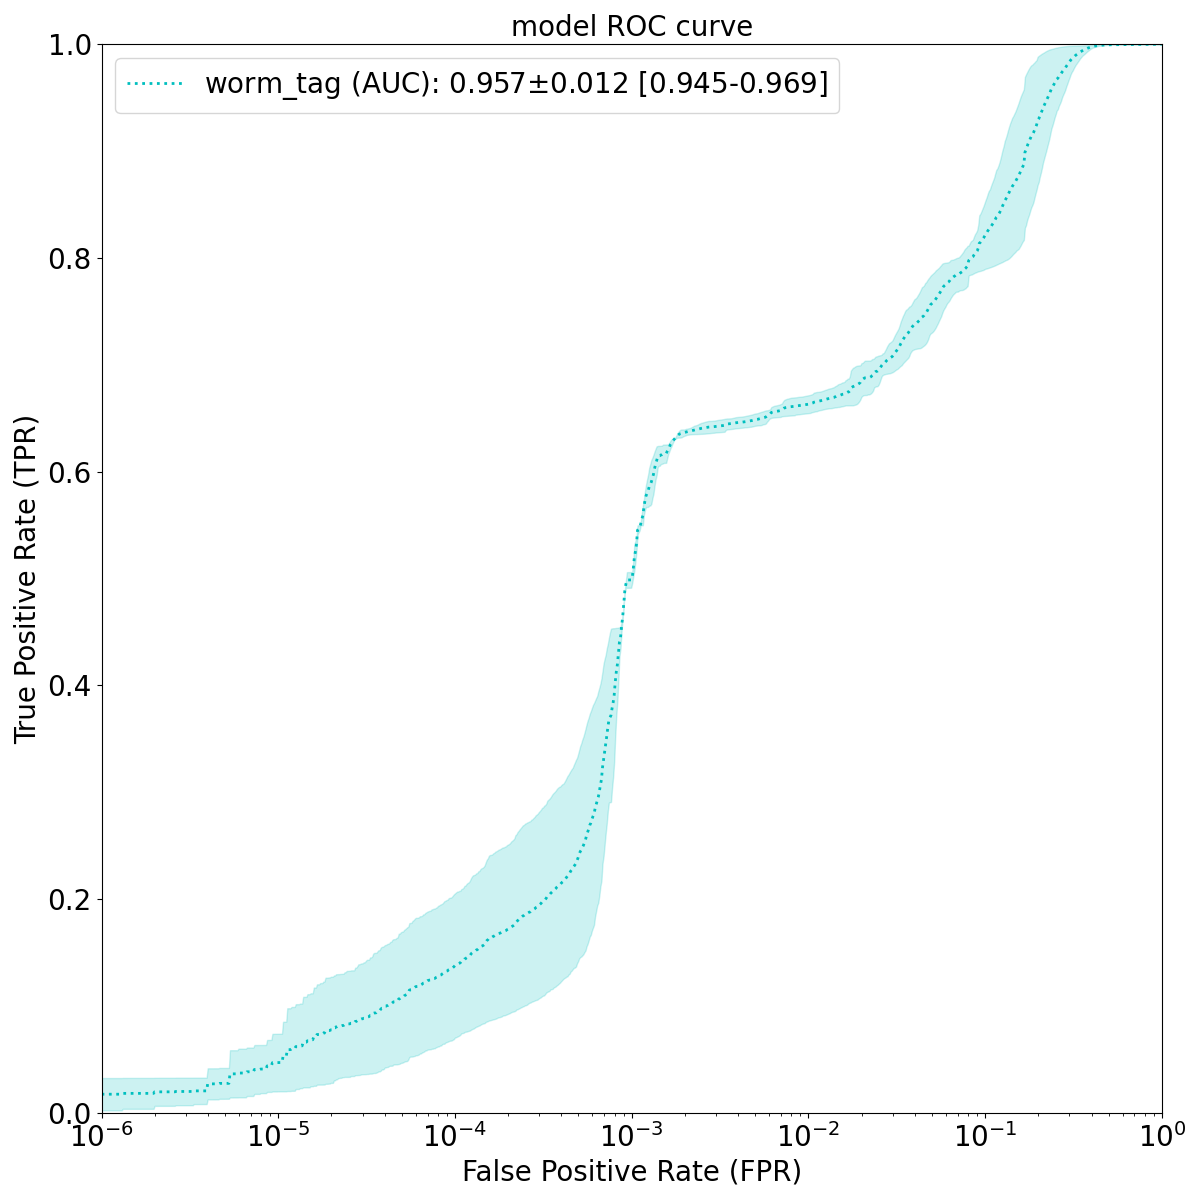
\includegraphics[width=0.6\textwidth]{./results/worm_tag_roc_jointEmbedding.png}
        \vspace*{-0.2cm}
        \caption[Worm Tag prediction task Joint Embedding ROC curve]{ROC curve and AUC statistics of \textBF{Joint Embedding} model for the \textbf{Worm Tag}. The line represents the \textit{mean} TPR at a given FPR, while the shaded region represents the \textit{standard deviation}. Statistics were computed over \textBF{3} training runs, each with random parameter initialization.}
        \label{fig:wormTagRocJointEmbedding}
    \end{figure}
}

\newcommand{\wormTagRocProposedMethod}{
    \begin{figure}[H]
        \vspace*{-0.5cm}
        \centering
        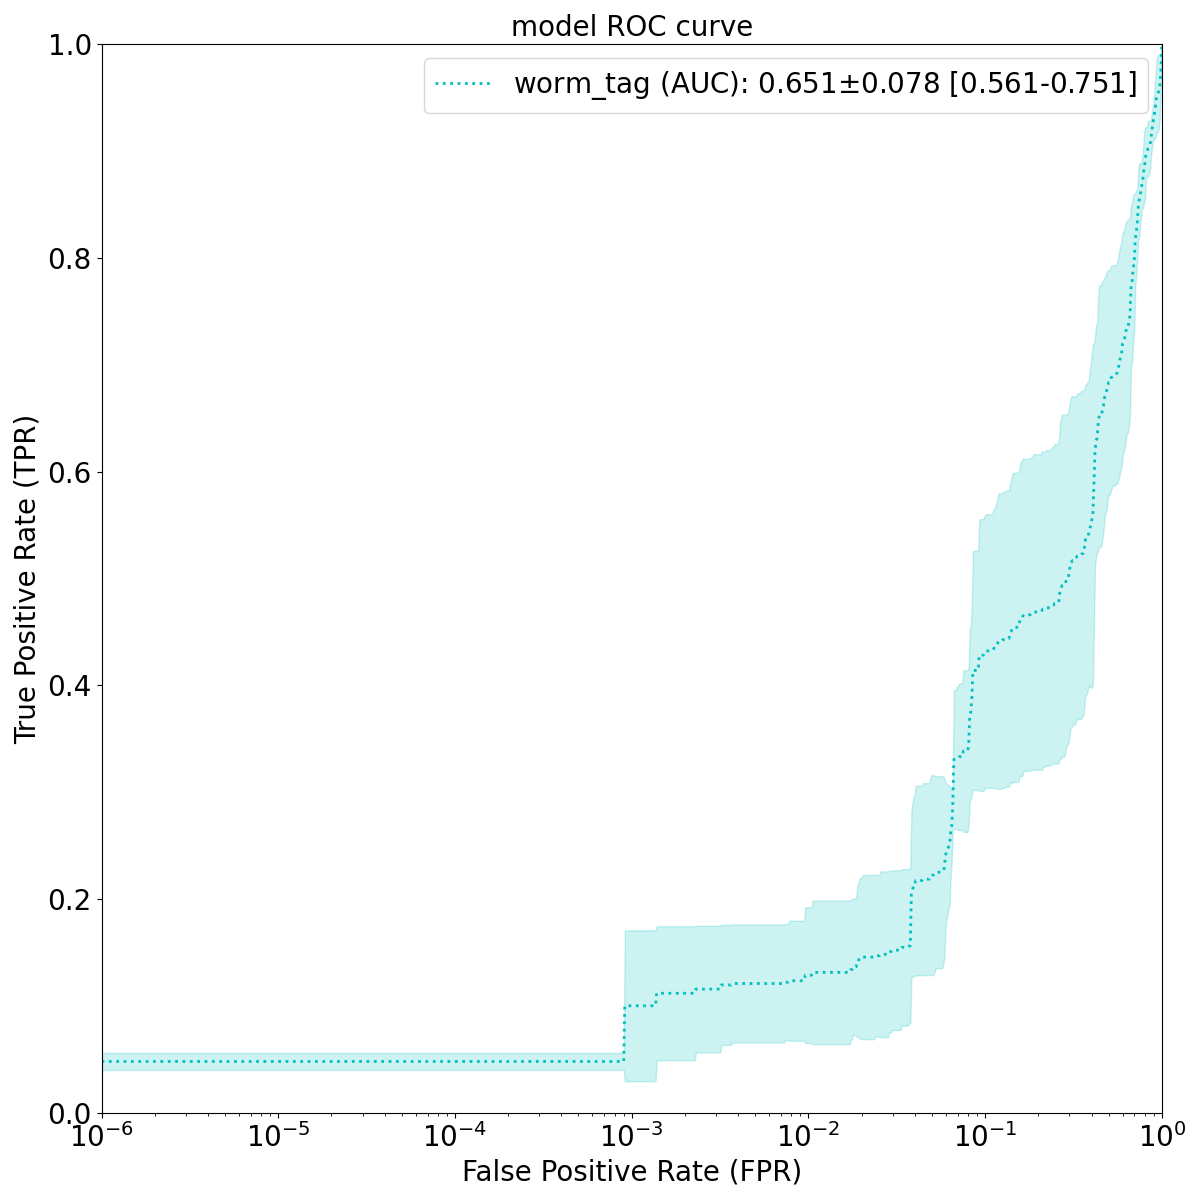
\includegraphics[width=0.6\textwidth]{./results/worm_tag_roc_proposedModel.png}
        \vspace*{-0.2cm}
        \caption[Worm Tag prediction task Proposed Model ROC curve]{ROC curve and AUC statistics of \textBF{Proposed Model} for the \textbf{Worm Tag}. The line represents the \textit{mean} TPR at a given FPR, while the shaded region represents the \textit{standard deviation}. Statistics were computed over \textBF{3} training runs, each with random parameter initialization.}
        \label{fig:wormTagRocProposedModel}
    \end{figure}
}
